\section{Biological and computational background}
\label{sec:fundamentals}

	\par Biological sensory systems convert external stimuli — such as light, odors, touch, and taste — into discrete electrical events known as \textbf{spikes}. A spike is a voltage pulse that conveys information through the nervous system \cite{kasabov2019time}. These signals are propagated along neural pathways to be processed, ultimately generating behavioral or physiological responses to the environment.
	
	\par A biological neuron emits a spike only when the accumulated excitatory input at the soma exceeds a certain threshold. In the absence of such stimulation, the neuron remains inactive. This event-driven behavior makes biological neurons highly efficient in terms of energy consumption and computational resources.
	
	\par Spiking Neural Networks (SNNs) aim to emulate some of these advantages by processing \textbf{spikes} at the input, hidden, and output layers. SNNs can also accept continuous-valued inputs retaining their event-driven properties and energy efficiency due to sparse activation patterns.
	
	\par It is important to note that SNNs are \textbf{not} detailed simulations of biological neurons. Instead, they approximate specific computational characteristics inspired by neurobiology. More biologically faithful models - such as the \textbf{Hodgkin–Huxley neuron} \cite{gerstner2014neuronal} and those explored in \cite{jones2020single}, which incorporate dendritic nonlinearities and other advanced neuronal features - have shown remarkable results in classification tasks, but at the cost of greater computational complexity.
	
	\par As illustrated in \autoref{fig:neuronspike}, SNN neurons exhibit strong noise tolerance when appropriately parameterized, functioning as \textbf{low-pass filters}. They can still generate reliable spikes under considerable interference. Moreover, SNN neurons are inherently time-sensitive, making them especially effective for processing temporal or sequential data streams \cite{10242251}.

	\begin{figure}[H]
		\centering
		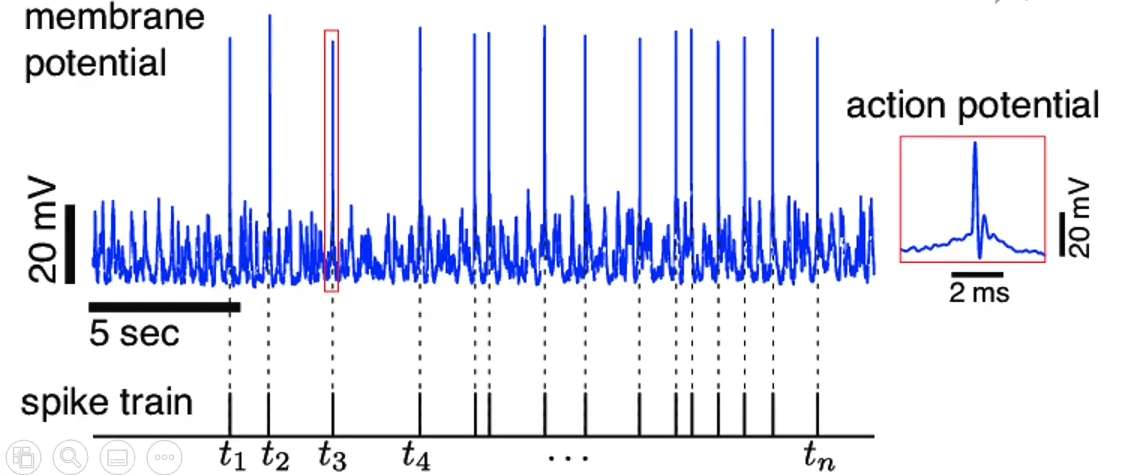
\includegraphics[width=\linewidth]{images/neuronSpikes}
		\caption{Spikes from a noisy signal: The noisy signal in blue is filtered generating sparse spikes. Source \cite{dan_goodman_2022_7044500}}
		\label{fig:neuronspike}
	\end{figure} 

	\subsection{\textbf{Leaky Integrate and Fire Neuron}}
	
		\par The focus of this work is the \textit{Leaky Integrate-and-Fire} (LIF) neuron due to its simplicity, computational efficiency, and its strong generalization performance across many tasks \cite{dan_goodman_2022_7044500}. 
		
		\par Unlike a standard artificial neuron, LIF integrates incoming weighted inputs over time with a \textit{leakage} mechanism that continuously reduces the membrane potential, simulating the passive decay observed in biological membranes. Only when the membrane potential crosses a threshold, does the neuron emit a spike, after which the potential resets or decreases.
		
		\par LIF behaves much like Resistor-Capacitor circuit like as illustrated in \autoref{fig:rcmodel}. 
		
		\begin{figure}[H]
			\centering
			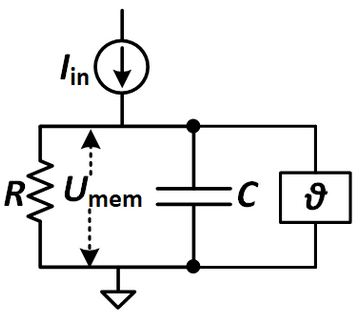
\includegraphics[width=0.4\linewidth]{images/rcmodel}
			\caption[The RC model with switch]{RC model with switch:
				$R$ represents the leakage resistance, $I_{in}$ the input current, $C$ the membrane capacitance, $U_{mem}$ the membrane potential (i.e., the accumulated charge) and $\vartheta$ a switch that lets the capacitor discharge (i.e. emit a spike) when a voltage threshold is reached.
				 Source: \cite{10242251}}
			\label{fig:rcmodel}
		\end{figure}
		
		\par Spikes are represented as \textbf{sparsely} distributed \textbf{ones} in a train of \textbf{zeros}, as illustrated in  \autoref{fig:spikessparsitystaticsupress} and \autoref{fig:sparsity}. This approach simplify the models and reduces the computational power and needed storage to run a SNN.\newline
		
		\begin{figure}[H]
			\centering
			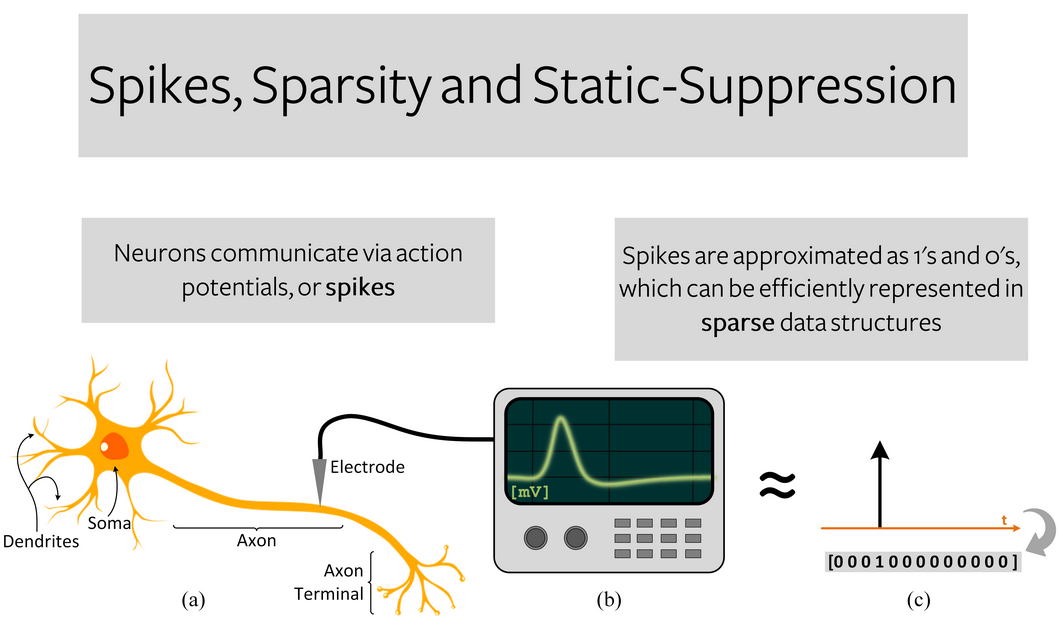
\includegraphics[width=\linewidth]{images/spikesSparsityStaticSupress}
			\caption{Sparsity on Spike Neuron Networks. Source: \cite{10242251}}
			\label{fig:spikessparsitystaticsupress}
		\end{figure}

		\begin{figure}[H]
			\centering
			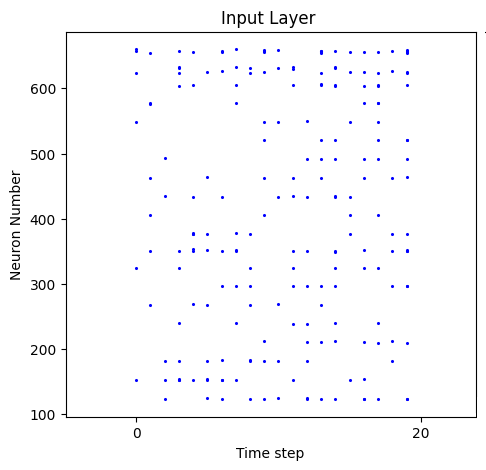
\includegraphics[width=.5\linewidth]{images/sparsity}
			\caption[Sparse activity of a SNN]{Sparse activity of a SNN: The horizontal axis represents the time step of some data being processed the vertical are the SNN neuron number. Note that, most of the time, very few neurons gets activated. Source: The author.}
			\label{fig:sparsity}
		\end{figure}
		
		\par As a result of the aforementioned characteristics, information in SNNs is encoded in terms of the \textit{timing} and/or \textit{rate} of spikes. This enables effective processing of temporal data streams but imposes limitations when dealing with static data like images which need some preprocessing in order to be better interpreted by a spiking neural network.\newline
		
		\par These preprocessing steps may consist of repeated copies of the input data for temporal reinforcement, or of a progressive decomposition of the input information, enabling its presentation in temporally distributed segments. 
		
	\subsection{\textbf{Mathematical Model of the LIF Neuron inner workings}}
	
			
		\par The first subsection presents an analytical study of the \textit{Resistor-Capacitor (RC) circuit model}, which governs the membrane potential dynamics of the LIF neuron, including both charging and discharging phases. Corresponding implementations and plots are provided. Building on this foundation, the second subsection focuses on implementing the complete LIF model, incorporating threshold mechanisms and potential resets.
		
		\subsubsection{\textbf{Membrane Charging and Discharging}}
		
			\par As shown in \autoref{fig:rcmodel}, a LIF neuron can be modeled as an RC circuit with a switch. By isolating the RC circuit, as illustrated in \autoref{fig:rcmodel2}, one can analyze the dynamics of membrane currents and potential governed by the equations described in \cite{10242251} and shown bellow:
		
			\begin{figure}[H]
				\centering
				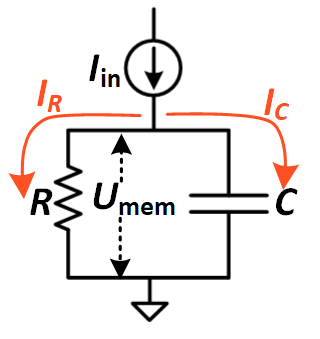
\includegraphics[width=0.4\linewidth]{images/rcmodel2}
				\caption[RC model for currents]{RC model for currents: $I_{in}(t) = I_R(t) + I_C(t)$}
				\label{fig:rcmodel2}
			\end{figure}
		
			\par Let's consider $Q$ as a measurement of electrical charge and $V_{mem}(t)$ is the membrane potential in a certain time $t$ than the neuron capacitance $C$ is given by \autoref{eq:capacitance}.
			
			\begin{equation}
				\label{eq:capacitance}
				C = \frac{Q}{V_{mem}(t)}
			\end{equation}
			
			\par Therefore the neuron charge can be expressed as \autoref{eq:charge}.
			
			\begin{equation}
				\label{eq:charge}
				Q = C.V_{mem}(t)
			\end{equation}
		
			\par To know how the charge changes according to the time (a.k.a. current) we can differentiate $Q$ as in \autoref{eq:rateOfChargeChange}. This is the expression of the electric current in the capacitive part of the neuron $I_C$.
			
			\begin{equation}
				\label{eq:rateOfChargeChange}
				\begin{aligned}
				I_C(t) = \dfrac{dQ}{dt} \implies \Aboxed{I_C(t) = C. \dfrac{dV_{mem}(t)}{dt}}
				\end{aligned}
			\end{equation}
		
		
			\par Then to calculate the total current passing by the resistive part $R$ of the circuit according to Ohm's law:
			
			\begin{equation}
				\label{eq:ohmlaw}
				\begin{aligned}
				V_{mem}(t) = R.I_R(t) \implies \Aboxed{I_R(t) = \frac{V_{mem}(t)}{R}}
				\end{aligned}
			\end{equation}
			
			\par Than considering that the total current do not change, as seen in \autoref{fig:rcmodel2}, then the total input current $I_{in}$ of the neuron can be expressed as in \autoref{eq:totalNeuronCurrent}.
			
			\begin{equation}
				\label{eq:totalNeuronCurrent}
				\begin{aligned}
				I_{in}(t) = I_R(t) + I_C(t) \implies \Aboxed{I_{in}(t) = \frac{V_{mem}(t)}{R} + C.\dfrac{dV_{mem}(t)}{dt}}
				\end{aligned}
			\end{equation}
			\par Therefore, to describe the passive membrane we got a linear  \autoref{eq:memLinear}.
			\begin{equation}
				\label{eq:memLinear}
				\begin{aligned}
					I_{in}(t) &= \frac{V_{mem}(t)}{R} + C.\dfrac{dV_{mem}(t)}{dt} \implies \\ 
					I_{in}(t) - \frac{V_{mem}(t)}{R} &=  C.\dfrac{dV_{mem}(t)}{dt} \implies \\
					\Aboxed{R.I_{in}(t) - V_{mem}(t) &=  R.C.\dfrac{dV_{mem}(t)}{dt}}
				\end{aligned}
			\end{equation}
	
			\par Defining $\tau = R C$ as the \textbf{membrane time constant}, we obtain \autoref{eq:finalMem}, which describes the RC circuit dynamics. This terminology arises from dimensional analysis: the right-hand side of the equation has units of \textit{voltage}, whereas the left-hand side contains $\dfrac{dV_{mem}(t)}{dt}$, which has units of \textit{voltage per time}. To maintain dimensional consistency, $R C$ must therefore have units of time.
	
			\begin{equation}
				\label{eq:finalMem}
				\begin{aligned}
				R.I_{in}(t) - V_{mem}(t) &=  R.C.\dfrac{dV_{mem}(t)}{dt} \implies \\
				R.I_{in}(t) - V_{mem}(t) &=  \tau.\dfrac{dV_{mem}(t)}{dt} \implies \\
				\Aboxed{\tau.\dfrac{dV_{mem}(t)}{dt} &= R.I_{in}(t) - V_{mem}(t)}
				\end{aligned}
			\end{equation}
			
			\par To model the \textbf{potential decay}, we set $I_{in}(t) = 0$ (i.e., no input) and assume $\tau = R C$ as constant with an initial membrane potential $V_{mem}(0) > 0$. Under these conditions, the membrane voltage follows an exponential decay, as shown in \autoref{eq:expmembrane}.
		
		 	\begin{equation}
		 		\label{eq:expmembrane}
		 		\begin{aligned}
		 		\tau.\dfrac{dV_{mem}(t)}{dt} &= R.I_{in}(t) - V_{mem}(t) \implies \\
		 		\tau.\dfrac{dV_{mem}(t)}{dt} &= R.0 - V_{mem}(t) \implies \\
		 		\tau.\dfrac{dV_{mem}(t)}{dt} &= -V_{mem}(t) = \\
		 		e^{\ln(V_{mem}(t))} &= e^{-\frac{t}{\tau}} = \\
		 		\Aboxed{V_{mem}(t) &= V_{mem}(0).e^{-\frac{t}{\tau}}}
		 		\end{aligned}
		 	\end{equation}
	 	
	 		\par In summary: In the absence of an input $I_{in}$, the membrane potential decays exponentially as illustrated in \autoref{fig:membranepotentialdecay} and implemented in  \autoref{lst:membranepotentialdecay}.
 		
 			\begin{lstlisting}[language=Python, caption={
		Python implementation of the action potential behavior of a LIF:
		\textbf{V\_mem}: Membrane potential at the current time step;
		\textbf{dt=1}: simulation time step;
		\textbf{I\_in=0}: No input current to the neuron;
		\textbf{R=5}: membrane resistance;
		\textbf{C=1}: membrane capacitance;
		\textbf{tau = R * C}: membrane time constant (i.e., the characteristic decay time of the membrane potential);
		\textbf{decay\_rate=-dt/tau}: The rate by which the membrane voltage decays for each time step.
		}, label={lst:membranepotentialdecay}]
def lif(V_mem, dt=1, I_in=0, R=5, C=1):
	tau = R*C
	
	# e^(-dt/tau)
	decay_rate = np.exp(-dt/tau)

	# V_mem(t) = V_mem(0) * e^(-dt/tau)
	V_mem = V_mem + (V_mem + I_in*R) * decay_rate

	return V_mem
\end{lstlisting}

	 		\begin{figure}[H]
	 			\centering
	 			
\includegraphics[width=\linewidth]{images/membranePotentialDecay}
	 			\caption{Membrane potential decaying when $I_{in} = 0$:
	 				Time is represented by the horizontal axis.
	 				Neuron charge in Volts is the vertical axis.
	 				Source: The author}
	 			\label{fig:membranepotentialdecay}
	 		\end{figure}
			
			\par With the results from \autoref{eq:finalMem} it is possible to calculate the action potential increasing as seen in \autoref{eq:actionpotincrease}.
			
			\begin{equation}
				\label{eq:actionpotincrease}
				\begin{aligned}
				&\tau.\dfrac{dV_{mem}(t)}{dt} = R.I_{in}(t) - V_{mem}(t) = \\
				&\dfrac{dV_{mem}(t)}{dt} + \frac{V_{mem}(t)}{\tau} = \frac{R.I_{in}(t)}{\tau} \implies \\
				&\text{Integrating factor: } e^{\int \frac{1}{\tau} dt} = e^{\frac{t}{\tau}} \implies \\
				&V_{mem}(t) = \dfrac{1}{e^{\frac{t}{\tau}}} . \left( \int \frac{R.I_{in}(t)}{\tau}.e^{\frac{t}{\tau}} dt \right) \therefore \\
				\Aboxed{&V_{mem}(t) = I_{in}(t).R(1-e^{\frac{-t}{\tau}})}
				\end{aligned}
			\end{equation}
			
			\par Note that, as seen in \autoref{fig:membranepotentialincrease} and implemented in \autoref{lst:membranepotentialincrease}, action potentials also increases exponentially.
			
			
 			\begin{lstlisting}[language=Python, caption={
		Python implementation of the increasing action potential behavior of a LIF:
		\textbf{V\_mem}: Membrane potential at the current time step;
		\textbf{t=1}: simulation time step;
		\textbf{R=5}: membrane resistance;
		\textbf{C=1}: membrane capacitance;
		\textbf{tau = R * C}: membrane time constant (i.e., the characteristic decay time of the membrane potential);
		\textbf{decay\_rate=-t/tau}: The rate by which the membrane voltage decays for each time step.
	}, label={lst:membranepotentialincrease}]
def lifIncrease(V_mem, t=1, I_in=1, R=5, C=1):    
	tau = R * C
	
	# e^(-dt/tau)
	decay_rate = np.exp(-t/tau)
	
	# V_mem(t)=I_in(t).R.(1 - e^(-t/tau))
	V_mem = V_mem + I_in * R * (1 - decay_rate)
	
	return V_mem
\end{lstlisting}
			
			
 			\begin{figure}[H]
 				\centering
 				
\includegraphics[width=\linewidth]{images/membranePotentialIncrease}
 				\caption{Membrane potential increasing when setting I\_in = 1 in \autoref{lst:membranepotentialincrease}:
 					Time is represented by the horizontal axis.
 					Neuron charge in Volts is the vertical axis.
 					Source: The author}
 				\label{fig:membranepotentialincrease}
 			\end{figure}
 			
		\subsubsection{\textbf{Implementation with Resets and Thresholds}}
			\label{sec:finalImplementation}
		
			\par Starting from \autoref{eq:finalMem}, we apply the forward Euler method to numerically solve for successive values of $V_{mem}$. This enables the construction of a fully functional LIF model.

			\begin{equation}
				\begin{aligned}
					\tau.\dfrac{dV_{mem}(t)}{dt} &= R.I_{in}(t) - V_{mem}(t) \implies \\
					\tau.\dfrac{V_{mem}(t + \Delta t) - V_{mem}(t)}{\Delta t} &= R.I_{in}(t) - V_{mem}(t) \implies \\
					V_{mem}(t + \Delta t) - V_{mem}(t) &= \dfrac{\Delta t}{\tau} (R.I_{in}(t) - V_{mem}(t)) \implies \\
					\Aboxed{V_{mem}(t + \Delta t) &= V_{mem}(t) + \dfrac{\Delta t}{\tau} (R.I_{in}(t) - V_{mem}(t))}
				\end{aligned}
			\end{equation}
		
			\par Now, introducing a \textbf{threshold} that triggers a reset of the membrane potential—either by resetting to zero or by subtracting the threshold value—allows us to model the complete charge and discharge behavior of the LIF neuron. This behavior is illustrated in \autoref{fig:membranepotentialfull} and implemented in \autoref{lst:membranepotentialfull}.

			\begin{lstlisting}[language=Python, caption={Python implementation of the action potential full simulation of a LIF:
	\textbf{V\_mem}: current membrane potential;
	\textbf{dt=1}: simulation time step;
	\textbf{I\_in=0.5}: input current (assumed constant during dt);
	\textbf{R=5}: membrane resistance;
	\textbf{C=}1: membrane capacitance;
	\textbf{V\_thresh=2}: firing threshold - when V\_mem > V\_thresh, the neuron "spikes";
	\textbf{reset\_zero=True}: determines if the neuron resets to zero after spiking;
	\textbf{tau = R * C}: membrane time constant (i.e., the characteristic decay time of the membrane potential);
	\textbf{decay\_rate=-dt/tau}: The rate by which the membrane voltage decays for each time step.
	}, label={lst:membranepotentialfull}]
def lif(V_mem, dt=1, I_in=0.5, R=5, C=1, V_thresh = 2, reset_zero = True):
	tau = R*C
	
	# e^(-dt/tau)
	decay_rate = np.exp(-dt/tau)
	
	# V_mem(t) = V_mem(0) * e^(-dt/tau)
	V_mem = V_mem + (V_mem + I_in*R) * decay_rate
	
	if V_mem > V_thresh:
		if reset_zero:
			V_mem = 0
		else:
			V_mem = V_mem - V_thresh
	return V_mem
\end{lstlisting}

			
			\begin{figure}[H]
				\centering
				
\includegraphics[width=\linewidth]{images/membranePotentialFull}
				\caption{Plot of the full simulated LIF: A 0.5 mA was provided from time 51 to 70.}
				\label{fig:membranepotentialfull}
			\end{figure}
 			
 	\subsection{\textbf{Training}}
 	
 		\par Until now just the \textit{forward} pass has been shown, it's time to describe the backwards.
 	
		\par As seen, the SNN neuron has an activation-function behavior that is more relatable to a \textbf{step function}. Therefore, in principle, we can't use gradient descent-based solutions because this kind of function \textbf{is not} differentiable \cite{kasabov2019time}.
		
		\par But there are some insights out there that may shed some light on this subject: While some \textit{in vivo/in vitro} observations show that brains, in general, learn by strengthening/weakening and adding/removing synapses or even by creating new neurons or other cumbersome methods like RNA packets, there are some more straightforward ways like the ones listed bellow \cite{kasabov2019time}:
 	
		\begin{itemize}
			\item \textbf{surrogate gradient descent(chosen)}: Approximates the step function by using another mathematical function, which is differentiable (like a sigmoid), in order to train the network. These approximations are used only in the backward pass, while keeping the step function in the forward pass \cite{kasabov2019time}.
			
			\item \textbf{Spike Timing-Dependent Plasticity (STDP)}: If a pre-synaptic neuron fires \textbf{before} the post-synaptic one, there is a strengthening in connection, but if the post-synaptic neuron fires before, then there is a weakening.

			\item \textbf{evolving algorithms}: Use the selection of the fittest throughout many generations of networks.
			
			\item \textbf{reservoir/dynamic Computing}: \textbf{Echo state networks} or \textbf{Liquid state machines} respectively.
		\end{itemize}
		
		\par As stated, the \textbf{surrogate gradient descent} method will be used, and the chosen approximated activation function is \textit{Hardtanh}, which is defined in \autoref{eq:hardtanh}, with its derivative given in \autoref{eq:dhardtanh}.
		
		\begin{equation}
			\label{eq:hardtanh}
			hardtanh(x) = 
			\begin{cases}
				maxVal, & x < maxVal\\
				minVal, & x > minVal\\
				x, & otherwise
			\end{cases}			
		\end{equation}
			
		\begin{equation}
			\label{eq:dhardtanh}
			\dfrac{d}{dx}hardtanh(x) = 
			\begin{cases}
				0, & x < maxVal\\
				0, & x > minVal\\
				1, & otherwise
			\end{cases}			
		\end{equation}
		
			
			
			
			
			
			
			
			
			




